% REV01 Thu 24 Jun 2021 06:34:48 WIB
% START Tue 04 May 2021 13:55:16 WIB

\chapter{XXX}

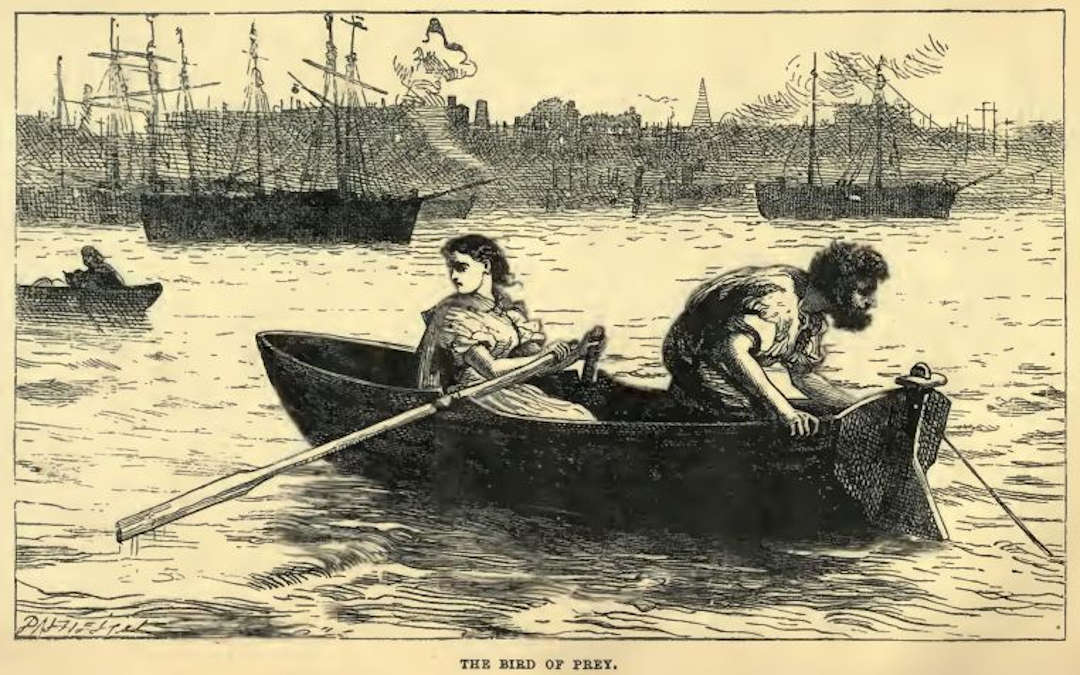
\includegraphics[scale=2.3]{01-01-01}

Chapter 4

A HAPPY RETURN OF THE DAY


Mr and Mrs Wilfer had seen a full quarter of a hundred more
anniversaries of their wedding day than Mr and Mrs Lammle had seen of
theirs, but they still celebrated the occasion in the bosom of
their family. Not that these celebrations ever resulted in anything
particularly agreeable, or that the family was ever disappointed by that
circumstance on account of having looked forward to the return of the
auspicious day with sanguine anticipations of enjoyment. It was kept
morally, rather as a Fast than a Feast, enabling Mrs Wilfer to hold
a sombre darkling state, which exhibited that impressive woman in her
choicest colours.

The noble lady’s condition on these delightful occasions was one
compounded of heroic endurance and heroic forgiveness. Lurid indications
of the better marriages she might have made, shone athwart the awful
gloom of her composure, and fitfully revealed the cherub as a little
monster unaccountably favoured by Heaven, who had possessed himself of a
blessing for which many of his superiors had sued and contended in vain.
So firmly had this his position towards his treasure become established,
that when the anniversary arrived, it always found him in an apologetic
state. It is not impossible that his modest penitence may have even gone
the length of sometimes severely reproving him for that he ever took the
liberty of making so exalted a character his wife.

As for the children of the union, their experience of these festivals
had been sufficiently uncomfortable to lead them annually to wish, when
out of their tenderest years, either that Ma had married somebody else
instead of much-teased Pa, or that Pa had married somebody else instead
of Ma. When there came to be but two sisters left at home, the daring
mind of Bella on the next of these occasions scaled the height of
wondering with droll vexation ‘what on earth Pa ever could have seen in
Ma, to induce him to make such a little fool of himself as to ask her to
have him.’

The revolving year now bringing the day round in its orderly sequence,
Bella arrived in the Boffin chariot to assist at the celebration. It was
the family custom when the day recurred, to sacrifice a pair of fowls
on the altar of Hymen; and Bella had sent a note beforehand, to intimate
that she would bring the votive offering with her. So, Bella and the
fowls, by the united energies of two horses, two men, four wheels, and a
plum-pudding carriage dog with as uncomfortable a collar on as if he
had been George the Fourth, were deposited at the door of the parental
dwelling. They were there received by Mrs Wilfer in person, whose
dignity on this, as on most special occasions, was heightened by a
mysterious toothache.

‘I shall not require the carriage at night,’ said Bella. ‘I shall walk
back.’

The male domestic of Mrs Boffin touched his hat, and in the act of
departure had an awful glare bestowed upon him by Mrs Wilfer, intended
to carry deep into his audacious soul the assurance that, whatever his
private suspicions might be, male domestics in livery were no rarity
there.

‘Well, dear Ma,’ said Bella, ‘and how do you do?’

‘I am as well, Bella,’ replied Mrs Wilfer, ‘as can be expected.’

‘Dear me, Ma,’ said Bella; ‘you talk as if one was just born!’

‘That’s exactly what Ma has been doing,’ interposed Lavvy, over the
maternal shoulder, ‘ever since we got up this morning. It’s all very
well to laugh, Bella, but anything more exasperating it is impossible to
conceive.’

Mrs Wilfer, with a look too full of majesty to be accompanied by any
words, attended both her daughters to the kitchen, where the sacrifice
was to be prepared.

‘Mr Rokesmith,’ said she, resignedly, ‘has been so polite as to place
his sitting-room at our disposal to-day. You will therefore, Bella, be
entertained in the humble abode of your parents, so far in accordance
with your present style of living, that there will be a drawing-room for
your reception as well as a dining-room. Your papa invited Mr Rokesmith
to partake of our lowly fare. In excusing himself on account of a
particular engagement, he offered the use of his apartment.’

Bella happened to know that he had no engagement out of his own room at
Mr Boffin’s, but she approved of his staying away. ‘We should only have
put one another out of countenance,’ she thought, ‘and we do that quite
often enough as it is.’

Yet she had sufficient curiosity about his room, to run up to it with
the least possible delay, and make a close inspection of its contents.
It was tastefully though economically furnished, and very neatly
arranged. There were shelves and stands of books, English, French, and
Italian; and in a portfolio on the writing-table there were sheets upon
sheets of memoranda and calculations in figures, evidently referring to
the Boffin property. On that table also, carefully backed with canvas,
varnished, mounted, and rolled like a map, was the placard descriptive
of the murdered man who had come from afar to be her husband. She shrank
from this ghostly surprise, and felt quite frightened as she rolled and
tied it up again. Peeping about here and there, she came upon a print, a
graceful head of a pretty woman, elegantly framed, hanging in the corner
by the easy chair. ‘Oh, indeed, sir!’ said Bella, after stopping to
ruminate before it. ‘Oh, indeed, sir! I fancy I can guess whom you
think THAT’S like. But I’ll tell you what it’s much more like--your
impudence!’ Having said which she decamped: not solely because she was
offended, but because there was nothing else to look at.

‘Now, Ma,’ said Bella, reappearing in the kitchen with some remains of a
blush, ‘you and Lavvy think magnificent me fit for nothing, but I intend
to prove the contrary. I mean to be Cook today.’

‘Hold!’ rejoined her majestic mother. ‘I cannot permit it. Cook, in that
dress!’

‘As for my dress, Ma,’ returned Bella, merrily searching in a
dresser-drawer, ‘I mean to apron it and towel it all over the front; and
as to permission, I mean to do without.’

‘YOU cook?’ said Mrs Wilfer. ‘YOU, who never cooked when you were at
home?’

‘Yes, Ma,’ returned Bella; ‘that is precisely the state of the case.’

She girded herself with a white apron, and busily with knots and pins
contrived a bib to it, coming close and tight under her chin, as if it
had caught her round the neck to kiss her. Over this bib her dimples
looked delightful, and under it her pretty figure not less so. ‘Now,
Ma,’ said Bella, pushing back her hair from her temples with both hands,
‘what’s first?’

‘First,’ returned Mrs Wilfer solemnly, ‘if you persist in what I cannot
but regard as conduct utterly incompatible with the equipage in which
you arrived--’

[‘Which I do, Ma.’)

‘First, then, you put the fowls down to the fire.’

‘To--be--sure!’ cried Bella; ‘and flour them, and twirl them round, and
there they go!’ sending them spinning at a great rate. ‘What’s next,
Ma?’

‘Next,’ said Mrs Wilfer with a wave of her gloves, expressive of
abdication under protest from the culinary throne, ‘I would recommend
examination of the bacon in the saucepan on the fire, and also of the
potatoes by the application of a fork. Preparation of the greens will
further become necessary if you persist in this unseemly demeanour.’

‘As of course I do, Ma.’

Persisting, Bella gave her attention to one thing and forgot the
other, and gave her attention to the other and forgot the third, and
remembering the third was distracted by the fourth, and made amends
whenever she went wrong by giving the unfortunate fowls an extra spin,
which made their chance of ever getting cooked exceedingly doubtful. But
it was pleasant cookery too. Meantime Miss Lavinia, oscillating between
the kitchen and the opposite room, prepared the dining-table in the
latter chamber. This office she (always doing her household spiriting
with unwillingness) performed in a startling series of whisks and bumps;
laying the table-cloth as if she were raising the wind, putting down
the glasses and salt-cellars as if she were knocking at the door, and
clashing the knives and forks in a skirmishing manner suggestive of
hand-to-hand conflict.

‘Look at Ma,’ whispered Lavinia to Bella when this was done, and they
stood over the roasting fowls. ‘If one was the most dutiful child in
existence (of course on the whole one hopes one is), isn’t she enough
to make one want to poke her with something wooden, sitting there bolt
upright in a corner?’

‘Only suppose,’ returned Bella, ‘that poor Pa was to sit bolt upright in
another corner.’

‘My dear, he couldn’t do it,’ said Lavvy. ‘Pa would loll directly. But
indeed I do not believe there ever was any human creature who could keep
so bolt upright as Ma, ‘or put such an amount of aggravation into one
back! What’s the matter, Ma? Ain’t you well, Ma?’

‘Doubtless I am very well,’ returned Mrs Wilfer, turning her eyes upon
her youngest born, with scornful fortitude. ‘What should be the matter
with Me?’

‘You don’t seem very brisk, Ma,’ retorted Lavvy the bold.

‘Brisk?’ repeated her parent, ‘Brisk? Whence the low expression,
Lavinia? If I am uncomplaining, if I am silently contented with my lot,
let that suffice for my family.’

‘Well, Ma,’ returned Lavvy, ‘since you will force it out of me, I must
respectfully take leave to say that your family are no doubt under
the greatest obligations to you for having an annual toothache on your
wedding day, and that it’s very disinterested in you, and an immense
blessing to them. Still, on the whole, it is possible to be too boastful
even of that boon.’

‘You incarnation of sauciness,’ said Mrs Wilfer, ‘do you speak like that
to me? On this day, of all days in the year? Pray do you know what
would have become of you, if I had not bestowed my hand upon R. W., your
father, on this day?’

‘No, Ma,’ replied Lavvy, ‘I really do not; and, with the greatest
respect for your abilities and information, I very much doubt if you do
either.’

Whether or no the sharp vigour of this sally on a weak point of Mrs
Wilfer’s entrenchments might have routed that heroine for the time, is
rendered uncertain by the arrival of a flag of truce in the person of
Mr George Sampson: bidden to the feast as a friend of the family, whose
affections were now understood to be in course of transference from
Bella to Lavinia, and whom Lavinia kept--possibly in remembrance of his
bad taste in having overlooked her in the first instance--under a course
of stinging discipline.

‘I congratulate you, Mrs Wilfer,’ said Mr George Sampson, who had
meditated this neat address while coming along, ‘on the day.’ Mrs Wilfer
thanked him with a magnanimous sigh, and again became an unresisting
prey to that inscrutable toothache.

‘I am surprised,’ said Mr Sampson feebly, ‘that Miss Bella condescends
to cook.’

Here Miss Lavinia descended on the ill-starred young gentleman with a
crushing supposition that at all events it was no business of his. This
disposed of Mr Sampson in a melancholy retirement of spirit, until the
cherub arrived, whose amazement at the lovely woman’s occupation was
great.

However, she persisted in dishing the dinner as well as cooking it, and
then sat down, bibless and apronless, to partake of it as an illustrious
guest: Mrs Wilfer first responding to her husband’s cheerful ‘For what
we are about to receive--’ with a sepulchral Amen, calculated to cast a
damp upon the stoutest appetite.

‘But what,’ said Bella, as she watched the carving of the fowls, ‘makes
them pink inside, I wonder, Pa! Is it the breed?’

‘No, I don’t think it’s the breed, my dear,’ returned Pa. ‘I rather
think it is because they are not done.’

‘They ought to be,’ said Bella.

‘Yes, I am aware they ought to be, my dear,’ rejoined her father, ‘but
they--ain’t.’

So, the gridiron was put in requisition, and the good-tempered cherub,
who was often as un-cherubically employed in his own family as if he had
been in the employment of some of the Old Masters, undertook to grill
the fowls. Indeed, except in respect of staring about him (a branch of
the public service to which the pictorial cherub is much addicted), this
domestic cherub discharged as many odd functions as his prototype; with
the difference, say, that he performed with a blacking-brush on the
family’s boots, instead of performing on enormous wind instruments and
double-basses, and that he conducted himself with cheerful alacrity to
much useful purpose, instead of foreshortening himself in the air with
the vaguest intentions.

Bella helped him with his supplemental cookery, and made him very happy,
but put him in mortal terror too by asking him when they sat down at
table again, how he supposed they cooked fowls at the Greenwich dinners,
and whether he believed they really were such pleasant dinners as people
said? His secret winks and nods of remonstrance, in reply, made the
mischievous Bella laugh until she choked, and then Lavinia was obliged
to slap her on the back, and then she laughed the more.

But her mother was a fine corrective at the other end of the table; to
whom her father, in the innocence of his good-fellowship, at intervals
appealed with: ‘My dear, I am afraid you are not enjoying yourself?’

‘Why so, R. W.?’ she would sonorously reply.

‘Because, my dear, you seem a little out of sorts.’

‘Not at all,’ would be the rejoinder, in exactly the same tone.

‘Would you take a merry-thought, my dear?’

‘Thank you. I will take whatever you please, R. W.’

‘Well, but my dear, do you like it?’

‘I like it as well as I like anything, R. W.’ The stately woman would
then, with a meritorious appearance of devoting herself to the general
good, pursue her dinner as if she were feeding somebody else on high
public grounds.

Bella had brought dessert and two bottles of wine, thus shedding
unprecedented splendour on the occasion. Mrs Wilfer did the honours of
the first glass by proclaiming: ‘R. W. I drink to you.

‘Thank you, my dear. And I to you.’

‘Pa and Ma!’ said Bella.

‘Permit me,’ Mrs Wilfer interposed, with outstretched glove. ‘No. I
think not. I drank to your papa. If, however, you insist on including
me, I can in gratitude offer no objection.’

‘Why, Lor, Ma,’ interposed Lavvy the bold, ‘isn’t it the day that made
you and Pa one and the same? I have no patience!’

‘By whatever other circumstance the day may be marked, it is not the
day, Lavinia, on which I will allow a child of mine to pounce upon me.
I beg--nay, command!--that you will not pounce. R. W., it is appropriate
to recall that it is for you to command and for me to obey. It is your
house, and you are master at your own table. Both our healths!’ Drinking
the toast with tremendous stiffness.

‘I really am a little afraid, my dear,’ hinted the cherub meekly, ‘that
you are not enjoying yourself?’

‘On the contrary,’ returned Mrs Wilfer, ‘quite so. Why should I not?’

‘I thought, my dear, that perhaps your face might--’

‘My face might be a martyrdom, but what would that import, or who should
know it, if I smiled?’

And she did smile; manifestly freezing the blood of Mr George Sampson
by so doing. For that young gentleman, catching her smiling eye, was so
very much appalled by its expression as to cast about in his thoughts
concerning what he had done to bring it down upon himself.

‘The mind naturally falls,’ said Mrs Wilfer, ‘shall I say into a
reverie, or shall I say into a retrospect? on a day like this.’

Lavvy, sitting with defiantly folded arms, replied (but not audibly),
‘For goodness’ sake say whichever of the two you like best, Ma, and get
it over.’

‘The mind,’ pursued Mrs Wilfer in an oratorical manner, ‘naturally
reverts to Papa and Mamma--I here allude to my parents--at a period
before the earliest dawn of this day. I was considered tall; perhaps I
was. Papa and Mamma were unquestionably tall. I have rarely seen a finer
women than my mother; never than my father.’

The irrepressible Lavvy remarked aloud, ‘Whatever grandpapa was, he
wasn’t a female.’

‘Your grandpapa,’ retorted Mrs Wilfer, with an awful look, and in an
awful tone, ‘was what I describe him to have been, and would have struck
any of his grandchildren to the earth who presumed to question it. It
was one of mamma’s cherished hopes that I should become united to a
tall member of society. It may have been a weakness, but if so, it was
equally the weakness, I believe, of King Frederick of Prussia.’ These
remarks being offered to Mr George Sampson, who had not the courage to
come out for single combat, but lurked with his chest under the table
and his eyes cast down, Mrs Wilfer proceeded, in a voice of increasing
sternness and impressiveness, until she should force that skulker
to give himself up. ‘Mamma would appear to have had an indefinable
foreboding of what afterwards happened, for she would frequently urge
upon me, “Not a little man. Promise me, my child, not a little man.
Never, never, never, marry a little man!” Papa also would remark to me
(he possessed extraordinary humour), “that a family of whales must not
ally themselves with sprats.” His company was eagerly sought, as may
be supposed, by the wits of the day, and our house was their continual
resort. I have known as many as three copper-plate engravers exchanging
the most exquisite sallies and retorts there, at one time.’ (Here Mr
Sampson delivered himself captive, and said, with an uneasy movement on
his chair, that three was a large number, and it must have been highly
entertaining.) ‘Among the most prominent members of that distinguished
circle, was a gentleman measuring six feet four in height. HE was NOT
an engraver.’ (Here Mr Sampson said, with no reason whatever, Of course
not.) ‘This gentleman was so obliging as to honour me with attentions
which I could not fail to understand.’ (Here Mr Sampson murmured that
when it came to that, you could always tell.) ‘I immediately announced
to both my parents that those attentions were misplaced, and that I
could not favour his suit. They inquired was he too tall? I replied it
was not the stature, but the intellect was too lofty. At our house,
I said, the tone was too brilliant, the pressure was too high, to be
maintained by me, a mere woman, in every-day domestic life. I well
remember mamma’s clasping her hands, and exclaiming “This will end in
a little man!”’ (Here Mr Sampson glanced at his host and shook his head
with despondency.) ‘She afterwards went so far as to predict that it
would end in a little man whose mind would be below the average, but
that was in what I may denominate a paroxysm of maternal disappointment.
Within a month,’ said Mrs Wilfer, deepening her voice, as if she were
relating a terrible ghost story, ‘within a-month, I first saw R. W. my
husband. Within a year, I married him. It is natural for the mind to
recall these dark coincidences on the present day.’

Mr Sampson at length released from the custody of Mrs Wilfer’s eye, now
drew a long breath, and made the original and striking remark that there
was no accounting for these sort of presentiments. R. W. scratched his
head and looked apologetically all round the table until he came to his
wife, when observing her as it were shrouded in a more sombre veil than
before, he once more hinted, ‘My dear, I am really afraid you are not
altogether enjoying yourself?’ To which she once more replied, ‘On the
contrary, R. W. Quite so.’

The wretched Mr Sampson’s position at this agreeable entertainment
was truly pitiable. For, not only was he exposed defenceless to the
harangues of Mrs Wilfer, but he received the utmost contumely at the
hands of Lavinia; who, partly to show Bella that she (Lavinia) could do
what she liked with him, and partly to pay him off for still obviously
admiring Bella’s beauty, led him the life of a dog. Illuminated on the
one hand by the stately graces of Mrs Wilfer’s oratory, and shadowed
on the other by the checks and frowns of the young lady to whom he
had devoted himself in his destitution, the sufferings of this young
gentleman were distressing to witness. If his mind for the moment reeled
under them, it may be urged, in extenuation of its weakness, that it
was constitutionally a knock-knee’d mind and never very strong upon its
legs.

The rosy hours were thus beguiled until it was time for Bella to have
Pa’s escort back. The dimples duly tied up in the bonnet-strings and the
leave-taking done, they got out into the air, and the cherub drew a long
breath as if he found it refreshing.

‘Well, dear Pa,’ said Bella, ‘the anniversary may be considered over.’

‘Yes, my dear,’ returned the cherub, ‘there’s another of ‘em gone.’

Bella drew his arm closer through hers as they walked along, and gave it
a number of consolatory pats. ‘Thank you, my dear,’ he said, as if
she had spoken; ‘I am all right, my dear. Well, and how do you get on,
Bella?’

‘I am not at all improved, Pa.’

‘Ain’t you really though?’

‘No, Pa. On the contrary, I am worse.’

‘Lor!’ said the cherub.

‘I am worse, Pa. I make so many calculations how much a year I must have
when I marry, and what is the least I can manage to do with, that I am
beginning to get wrinkles over my nose. Did you notice any wrinkles over
my nose this evening, Pa?’

Pa laughing at this, Bella gave him two or three shakes.

‘You won’t laugh, sir, when you see your lovely woman turning haggard.
You had better be prepared in time, I can tell you. I shall not be able
to keep my greediness for money out of my eyes long, and when you see it
there you’ll be sorry, and serve you right for not being warned in time.
Now, sir, we entered into a bond of confidence. Have you anything to
impart?’

‘I thought it was you who was to impart, my love.’

‘Oh! did you indeed, sir? Then why didn’t you ask me, the moment we came
out? The confidences of lovely women are not to be slighted. However, I
forgive you this once, and look here, Pa; that’s’--Bella laid the
little forefinger of her right glove on her lip, and then laid it on her
father’s lip--‘that’s a kiss for you. And now I am going seriously
to tell you--let me see how many--four secrets. Mind! Serious, grave,
weighty secrets. Strictly between ourselves.’

‘Number one, my dear?’ said her father, settling her arm comfortably and
confidentially.

‘Number one,’ said Bella, ‘will electrify you, Pa. Who do you think
has’--she was confused here in spite of her merry way of beginning ‘has
made an offer to me?’

Pa looked in her face, and looked at the ground, and looked in her face
again, and declared he could never guess.

‘Mr Rokesmith.’

‘You don’t tell me so, my dear!’

‘Mis--ter Roke--smith, Pa,’ said Bella separating the syllables for
emphasis. ‘What do you say to THAT?’

Pa answered quietly with the counter-question, ‘What did YOU say to
that, my love?’

‘I said No,’ returned Bella sharply. ‘Of course.’

‘Yes. Of course,’ said her father, meditating.

‘And I told him why I thought it a betrayal of trust on his part, and an
affront to me,’ said Bella.

‘Yes. To be sure. I am astonished indeed. I wonder he committed himself
without seeing more of his way first. Now I think of it, I suspect he
always has admired you though, my dear.’

‘A hackney coachman may admire me,’ remarked Bella, with a touch of her
mother’s loftiness.

‘It’s highly probable, my love. Number two, my dear?’

‘Number two, Pa, is much to the same purpose, though not so
preposterous. Mr Lightwood would propose to me, if I would let him.’

‘Then I understand, my dear, that you don’t intend to let him?’

Bella again saying, with her former emphasis, ‘Why, of course not!’ her
father felt himself bound to echo, ‘Of course not.’

‘I don’t care for him,’ said Bella.

‘That’s enough,’ her father interposed.

‘No, Pa, it’s NOT enough,’ rejoined Bella, giving him another shake or
two. ‘Haven’t I told you what a mercenary little wretch I am? It
only becomes enough when he has no money, and no clients, and no
expectations, and no anything but debts.’

‘Hah!’ said the cherub, a little depressed. ‘Number three, my dear?’

‘Number three, Pa, is a better thing. A generous thing, a noble thing, a
delightful thing. Mrs Boffin has herself told me, as a secret, with her
own kind lips--and truer lips never opened or closed in this life, I am
sure--that they wish to see me well married; and that when I marry with
their consent they will portion me most handsomely.’ Here the grateful
girl burst out crying very heartily.

‘Don’t cry, my darling,’ said her father, with his hand to his eyes;
‘it’s excusable in me to be a little overcome when I find that my dear
favourite child is, after all disappointments, to be so provided for
and so raised in the world; but don’t YOU cry, don’t YOU cry. I am very
thankful. I congratulate you with all my heart, my dear.’ The good soft
little fellow, drying his eyes, here, Bella put her arms round his neck
and tenderly kissed him on the high road, passionately telling him
he was the best of fathers and the best of friends, and that on her
wedding-morning she would go down on her knees to him and beg his pardon
for having ever teased him or seemed insensible to the worth of such
a patient, sympathetic, genial, fresh young heart. At every one of her
adjectives she redoubled her kisses, and finally kissed his hat off, and
then laughed immoderately when the wind took it and he ran after it.

When he had recovered his hat and his breath, and they were going on
again once more, said her father then: ‘Number four, my dear?’

Bella’s countenance fell in the midst of her mirth. ‘After all, perhaps
I had better put off number four, Pa. Let me try once more, if for never
so short a time, to hope that it may not really be so.’

The change in her, strengthened the cherub’s interest in number four,
and he said quietly: ‘May not be so, my dear? May not be how, my dear?’

Bella looked at him pensively, and shook her head.

‘And yet I know right well it is so, Pa. I know it only too well.’

‘My love,’ returned her father, ‘you make me quite uncomfortable. Have
you said No to anybody else, my dear?’

‘No, Pa.’

‘Yes to anybody?’ he suggested, lifting up his eyebrows.

‘No, Pa.’

‘Is there anybody else who would take his chance between Yes and No, if
you would let him, my dear?’

‘Not that I know of, Pa.’

‘There can’t be somebody who won’t take his chance when you want him
to?’ said the cherub, as a last resource.

‘Why, of course not, Pa,’ said Bella, giving him another shake or two.

‘No, of course not,’ he assented. ‘Bella, my dear, I am afraid I must
either have no sleep to-night, or I must press for number four.’

‘Oh, Pa, there is no good in number four! I am so sorry for it, I am so
unwilling to believe it, I have tried so earnestly not to see it, that
it is very hard to tell, even to you. But Mr Boffin is being spoilt by
prosperity, and is changing every day.’

‘My dear Bella, I hope and trust not.’

‘I have hoped and trusted not too, Pa; but every day he changes for
the worse, and for the worse. Not to me--he is always much the same
to me--but to others about him. Before my eyes he grows suspicious,
capricious, hard, tyrannical, unjust. If ever a good man were ruined by
good fortune, it is my benefactor. And yet, Pa, think how terrible the
fascination of money is! I see this, and hate this, and dread this, and
don’t know but that money might make a much worse change in me. And yet
I have money always in my thoughts and my desires; and the whole life I
place before myself is money, money, money, and what money can make of
life!’



